\newpage
\chapter{Interesting thoughts and interpretations of dark matter (29/09/2016)}

\begin{easylist}[itemize]
\ListProperties(Style*=-- , FinalMark={)})

& Thought to be made of a neutral, weakly interacting particle. Because it's neutral (and thought to be elementary), it cannot couple to the electromagnetic field, so there's no way to detect it through conventional astronomy.

& Galaxies form and condense in dark matter wells because the baryonic matter does not produce a gravitational field strong enough to keep ahold of ordinary matter.

& Dark matter is not super dense (like a black hole around the centre of a galaxy). It is more "sprinkled" in a roughly-spherical halo throughout a galaxy. \cite{1970ApJ-160-811F,1992AandA-256-19B} Its average density is still much greater than that of the normal matter in the galaxy because it's the dark matter that leads to the flat rotation curve of most galaxies. \cite{1996MNRAS-281-27P} If there were only baryonic matter, the rotation curve would drop off as $\propto 1/\sqrt{r}$ as Kepler's laws state. Whilst the surface density of dark matter does decrease with radius -- so the density in a thin spherical shell around the galaxy decreases -- its inclusive mass increases linearly (see Figure 1 in \cite{2009arXiv0901.0632E}) to compensate for the Keplerian drop off in the baryonic matter (think Gauss' law). \cite{1972ApJ-176-1G,2006AJ-132-2685M} The dark matter "orbits" the centre of the galaxy \underline{with} the stars, but in some models has a lower velocity because it's angular momentum doesn't dissipate via collisions and collapse into a disc like baryonic matter does (because collisions would result in annihilation). In other models, it's corotational with the stars.

& Dark matter particles must be stable because they've existed for billions of years and have allowed galaxies to form in their potential wells.

& It is thought that dark matter was produced thermally in the early universe (when it was hot and therefore easier to create heavy particles). Dark matter particles could (and did) annihilate, but as the universe expanded and cooled the dark matter became more diffuse. They didn't annihilate as often and the dark matter we see today is a "thermal relic" and is what's left over. Some models suggest the parameter $x = m_{\mathrm{DM}}/T \sim 20$ at freeze out. \cite{Lisanti:2016jxe} 

& The current leading dark matter candidate is a WIMP (Weakly Interacting Massive Particle), possibly a neutral supersymmetric particle (neutralino) like a higgsino, photino, zino, etc. One of the motivations for WIMPs are that, using the current values of the dark matter density in the universe and approximations for the annihilation cross section, dark matter could self-interact at the electroweak scale to produce Standard Model particles. \cite{Kamionkowski:1997zb} As the EW scale can be readily accessed at colliders like the LHC, we could detect DM signatures via pair production then annihilation or indirect searches via solely annihilation.

& WIMP annihilation could produce two showers of quarks, which would normally be observed as pions and high energy photons (like gamma rays). The photons may be of a continuum -- from hadronisation and radiation of the decay products of annihilation -- or contain features (internal radiation from the propagator in the interaction or from loop-level processes).

& Because WIMPs are stable (at least on the timescale of the current age of the Universe), they wouldn't decay into other particles when produced from accelerator collisions. So you would detect them (indirectly) by looking for missing transverse momentum (\cancel{$p$}\textsubscript{T} or $\ptmiss$) or missing transverse energy (\cancel{$E$}\textsubscript{T} or \etmiss) and by looking for visible particles recoiling against the WIMPs.

& The mediator (force-carrying particle, like the gauge bosons) for dark matter -- between dark matter particles or the dark matter-Standard Model particle interactions -- may be a scalar (spin-0, like the Higgs boson) or pseudoscalar (reverses parity under a Lorentz transformation, like the pion) boson. [Support] for a pseudoscalar over a scalar mediator comes from the Feynman diagrams for DM annihilation into, e.g., $b$-quarks. With a scalar mediator, the vertex factors and the propagator term lead to cancellations in the cross section equation in the low-velocity limit.

& The mediator for dark matter may be heavier than the dark matter particle itself (like with the $W^{\pm}$ and $Z$ bosons being heavier than most of the particles they mediate), maybe 2x heavier or more so than the DM particle. The mediator could decay via DM pair production, so it makes sense that it would be at least twice as heavy.

& There's no consensus on whether dark matter is fermionic or bosonic. If fermionic, it may be either a Dirac fermion (particle is distinct from its antiparticle, like the electron and positron) or Majorana fermion (particle is the same as its antiparticle, like the neutrino is \underline{suspected} to be). If it were Majorana, dark matter could annihilate with itself, making discoveries via indirect searches more likely.

& At the LHC, monojets are used most prominently to look for dark matter particles. But multijet plus \etmiss might provide better sensitivity and constraints (particularly if the mediator is pseudoscalar).

& The Coma Cluster of galaxies seems to contain a very high concentration of dark matter (mass-to-light ratio of 400 $M_{\odot} / L_{\odot}$). See \cite{Yozin:2015mla}.

& \underline{Many} dark matter candidates include a few supersymmetric particles (the neutralino being the most widely studied), sterile neutrinos \cite{doi:10.1142/S0218301313300191}, axions, Kaluza-Klein states \cite{Han:1998sg} (which are excitations of Standard Model fields in extra dimensions), etc.

& Dark matter has to be cold (non-relativistic), as opposed to hot (relativistic), implying dark matter particles are reasonably heavy. If dark matter was light, it would have a lot of energy when produced in the early universe and would be relativistic (so hot). But if it were hot, it would be too diffusive to allow galaxies to form. However, because of the seemingly bottom-up nature of structure formation in the Universe \cite{doi:10.1093-mnras-183.3.341} (smaller galaxies form first around clumps of dark matter, then orbit and merge with other galaxies to form clusters and larger elliptical galaxies), dark matter must be cold so it doesn't diffuse too much and can clump to allow galaxy formation.

& The different aspects of dark matter searches:
\begin{figure}[H]
\centering
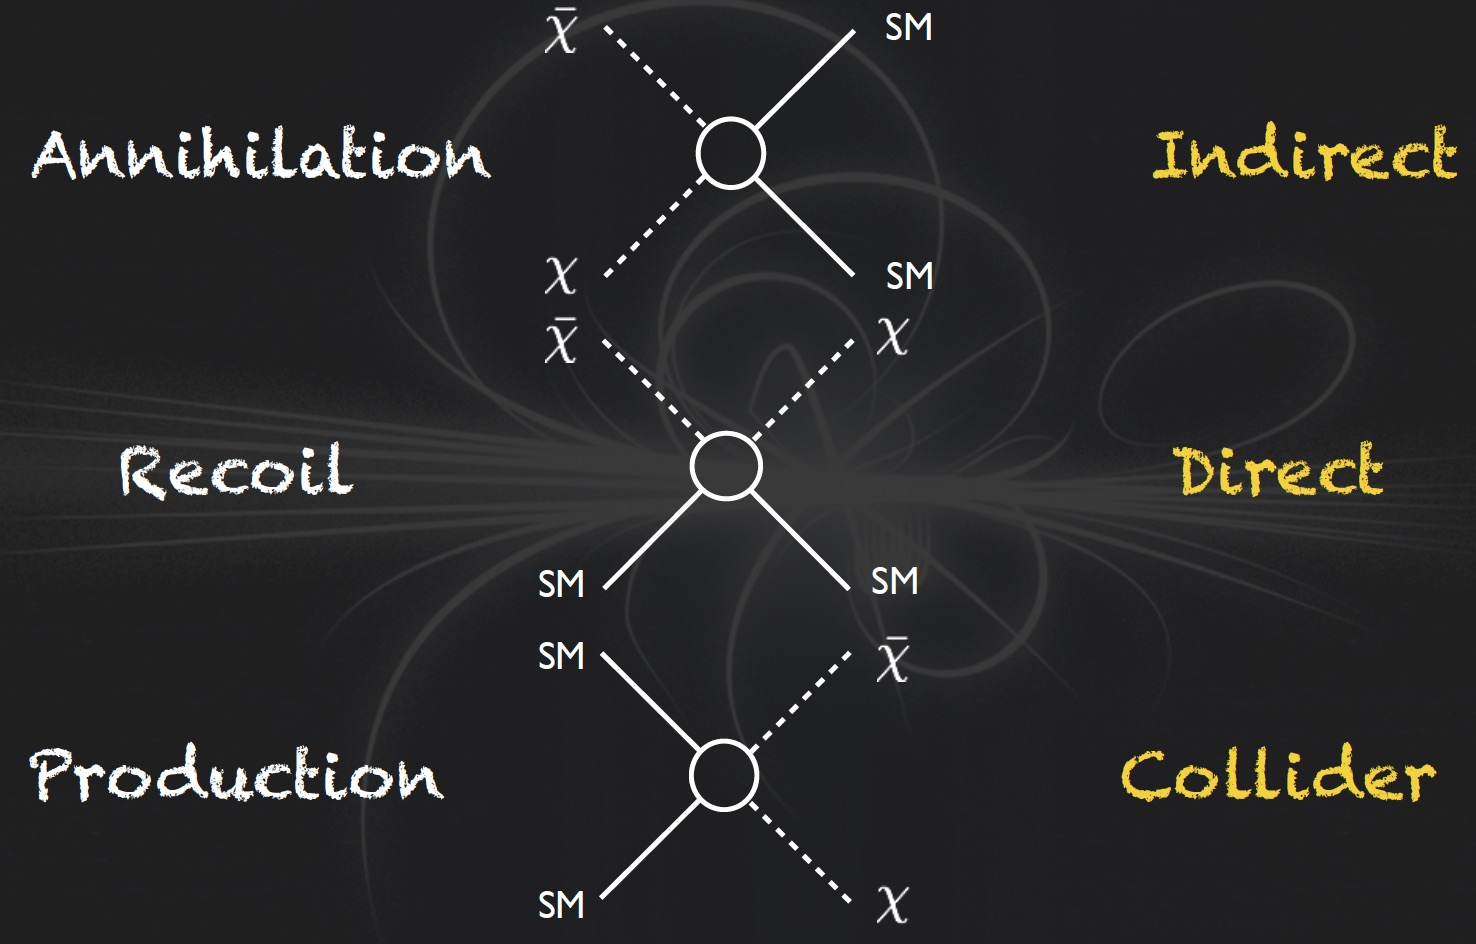
\includegraphics[width=\textwidth]{./sec5/Dark_matter_searches.jpg}
\caption{The different aspects of dark matter searches: indirect (annihilation), direct (scattering from SM particles), and collider (production). Taken from Bjoern's University of Wisconsin -- Madison talk, 27/03/2017.}
\end{figure}

& Some good results showcasing dark matter masses and that of its mediator from different analyses and decay channels are at \cite{CMS-DP-2016-057}. Particularly figures 4 and 6, which I used in my poster for the PGR conference.

& The 2015 results from Planck estimate the dark matter content of the universe to be 25.8\%. It displays it in terms of $\Omega_c h^2 = 0.1186$, where $h = 0.678$ (the Hubble constant, in units of km s$^{-1}$ Mpc$^{-1} / 100$), giving $\Omega_c = 0.258$ as the cold dark matter density \cite{2016AnA...594A..13P}.

& Dark matter cannot be solely neutrinos because the flux densities of neutrinos (from stars, as well as the cosmic neutrino background \cite{weinberg2008cosmology}) are precise and well-known, and due to the upper limit on neutrino masses \cite{Mertens:2016ihw}, are too small to account for the dark matter content in the universe. Because the neutrinos have such a small mass, they would be highly relativistic in the early universe (as they are today, despite it being cooler now, making them slower) and so could only contribute to hot dark matter \cite{Quigg:2008ab}. But as experiments show, the vast majority of dark matter must be cold.

& MOND (Modified Newtonian Dynamics) is one theory that tries to explain dark matter, and can be constrained to explain galactic rotation curves and other astrophysical phenomena attributed to it. However, any certain strand that tries to explain one observation usually falls flat when trying to explain others. It also doesn't work at all the scales to which we can observe the effects of General Relativity, almost confirming that GR is the correct description of gravity and MOND is a failure.

& LUX (Large Underground Xenon experiment) and LZ (LUX-Zeplin) are direct detection experiments that search explicitly for WIMP dark matter. LUX uses an underground liquid xenon tank to detect WIMPs interacting with ordinary matter, the scattering producing photons and electrons of specific energies. LZ is a collaboration between the LUX and ZEPLIN groups, and will have a highly-sensitive WIMP detector over a large range of masses, once completed.

& Evidence for non-luminous, \emph{non-baryonic} matter (an argument for those who ask why dark matter can't be neutrons, etc.):

One can use Doppler shifts of light emitted from galaxies in clusters, and therefore determine their masses. Then using the mass-to-light ratios of these galaxies and clusters (e.g., Bullet Cluster \cite{BulletClusterDMevidence}), one can determine that most of the mass comes from non-luminous matter \cite{cox2016universal}.

One can also use the Cosmic Microwave Background to calculate the average photon and neutrino (mass/energy) densities and Big Bang Nucleosynthesis calculations to determine the baryonic matter density. These can be compared to other measurements (e.g, mass-to-light ratios averaged across the universe) and reveal the discrepancy \cite{cox2016universal}.

Neutrons can't contribute to dark matter because isolated neutrons are unstable, decaying in a matter of minutes \cite{PDGbooklet2010}. They decay into protons and electrons. Being charged, they interact strongly with light and therefore contribute to the luminous matter in the universe.

\end{easylist}
